\section{Fourier Transformation}
\[
\boxed{f(t) =  \frac{1}{2\pi}\int\limits_{-\infty}^{\infty}
F(\omega)e^{j\omega t}d\omega}=\frac{1}{2
\pi}\int\limits_{-\infty}^{\infty}(R(\omega) \cos(\omega t) + X(\omega)
\sin(\omega t))d\omega + \frac{j}{2 \pi}\int \limits_{-
\infty}^{\infty}(R(\omega) \sin(\omega t)- X(\omega) \cos(\omega t))d\omega
\]

\[	
\boxed{F(\omega) = \int\limits_{-\infty}^{\infty} f(t)e^{-j\omega t}dt}
= R(\omega) - j X(\omega) \quad R(\omega) = \int\limits_{-\infty}^{\infty}
f(t)\cos(\omega t)dt \quad \mbox{ und } \quad X(\omega)=
\int\limits_{-\infty}^{\infty}f(t)\sin(\omega t)dt 
\]

\subsection{Spektren}
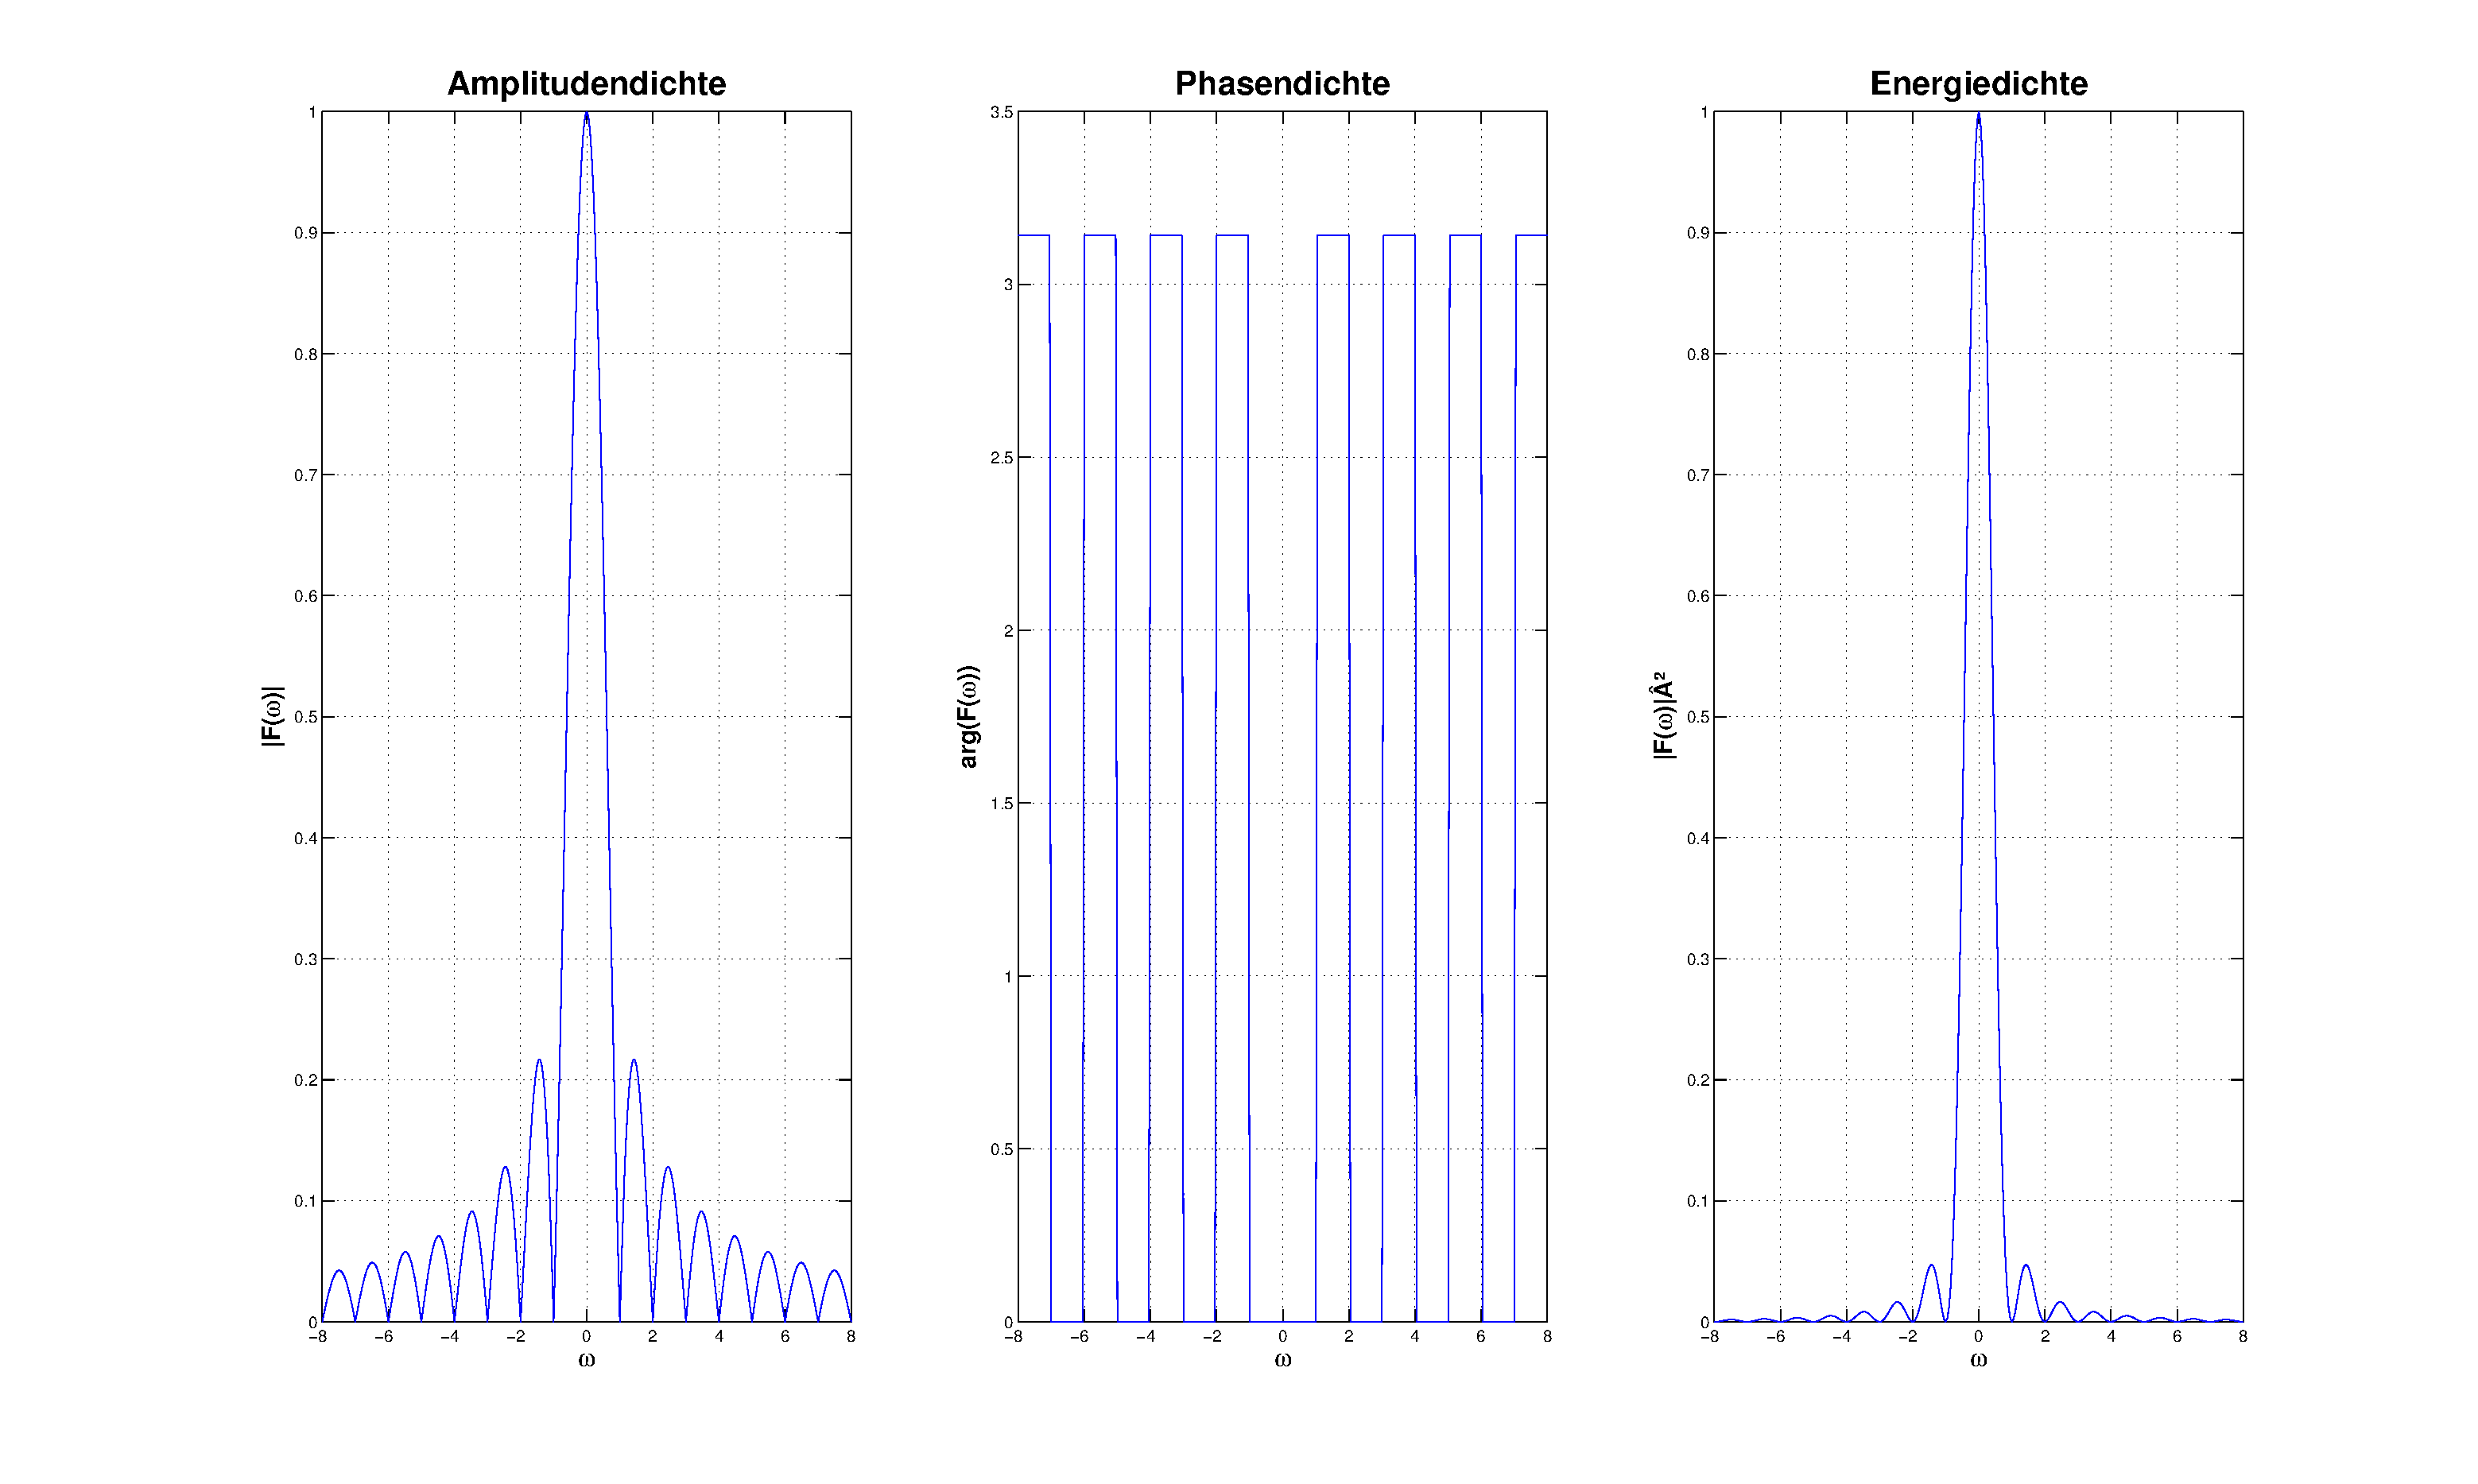
\includegraphics[width=0.8\textwidth,trim=1cm 1cm 1cm 1cm]{content/appendix/Spektern.pdf}

\newpage	
\subsection{Eigenschaften}
Fourierintegral existiert wenn  $\int\limits_{-\infty}^{\infty}|f(t)| dt < \infty$\\

\renewcommand{\arraystretch}{2}

\begin{tabular}{|p{8cm}|l c l|}
  \hline
 	Linearität & 
 	$\alpha\cdot f(t) + \beta\cdot g(t)$ & $\FT$ & $\alpha\cdot F(\omega) + \beta\cdot G(\omega)$\\
 	\hline
  Zeitumkehrung (Spiegelung an der Y-Achse)&
  $f(-t)$ & $\FT$ & $F(-\omega) = F^*(\omega)$ \\
	\hline        	
	Ähnlichkeit &
	$f(\alpha t)$ & $\FT$ & $\frac{1}{|\alpha|}F \left (\frac{\omega}{\alpha} \right) \quad\alpha \in\mathbb{R}\setminus \{0\}$\\
	\hline
	Verschiebung im	Zeitbereich &
	$f(t\pm t_0)$ & $\FT$ & $F(\omega)e^{\pm j\omega t_0}$\\
	\hline
  Verschiebung im Frequenzbereich &
	$f(t)e^{\pm j\omega_0 t}$ & $\FT$ & $F(\omega\mp\omega_0)$\\
	\hline
	Ableitung im Zeitbereich &
	$\frac{\partial^n f(t)}{\partial t^n}$ & $\FT$ & $(j\omega)^n F(\omega)$\\
	\hline
	Integration im Zeitbereich &
	$\int\limits_{-\infty}^{t}f(\tau)d\tau $ & $\FT$ & 
	$\frac{F(\omega)}{j\omega}+\pi F(0)\delta(\omega)$\\
	\hline				
	Ableitung im Frequenzbereich &
	$t^n f(t)$ & $\FT$ & $j^n \frac{\partial F(\omega)}{\partial \omega^n}$\\
	\hline		
	Faltung im Zeitbereich &
	$f(t) \ast g(t)$ & $\FT$ & $F(\omega) \cdot G(\omega)$\\
	\hline
	Faltung im Frequenzbereich &
	$f(t) \cdot g(t)$ & $\FT$ & $\frac{1}{2\pi}F(\omega) \ast G(j\omega)$\\
	\hline
	Vertauschungssatz (Dualität) &
	$f(t)$ & $\FT$ & $F(\omega)\nonumber$ \\
	& $F(t)$ & $\FT$ & $2\pi \cdot f(-\omega)$\\
	\hline
	Modulation &
	$\cos(\alpha t) \cdot f(t)$ & $\FT$ & $\frac{1}{2}\cdot \left[F(\omega-\alpha) + F(\omega+\alpha)\right ]$\\
	& $\sin(\alpha t) \cdot f(t)$ & $\FT$ & $\frac{1}{2j}\cdot \left[	F(\omega-\alpha) - F(\omega+\alpha)\right ]$\\
	\hline
 	Parseval's Theorem &
  $\int\limits_{-\infty}^{\infty}f(t)g^{\ast}(t)dt $ & $=$ & $ \frac{1}{2\pi}	\int\limits_{-\infty}^{\infty}F(\omega)G^{\ast}(\omega)d\omega$\\
	\hline
	Bessel's Theorem (Satz von Parseval) &
	$\int\limits_{-\infty}^{\infty}|f(t)|^2 dt $ & $=$ & $ \frac{1}{2\pi}\int\limits_{-\infty}^{\infty}|F(\omega)|^2 d\omega$\\
	\hline 			
  Anfangswerte &
  $f(0)=\frac{1}{2\pi}\int\limits_{-\infty}^{\infty}F(\omega)d\omega$ 
  && $ F(0)=\int\limits_{-\infty}^{\infty}f(t)dt$\\
	\hline
	$\infty$ lange Folge von $\delta$-Impulsen &
	$\sum\limits_{n=-\infty}^{\infty} \delta(t-n\cdot t_0)$ & $\FT$ & 
	$\sum\limits_{n=-\infty}^{\infty} \frac{2\pi}{t_0}\delta(\omega-n\cdot \frac{2\pi}{t_0})$\\
	\hline
\end{tabular}
\renewcommand{\arraystretch}{1}


\subsection{Wichtige Fourier Transformationspaare}
\begin{landscape}
\begin{center}
\renewcommand{\arraystretch}{2.5}
\begin{tabular}{|rll|rll|}
\hline
    $x(t)$ & $\FT$ & $X(\omega)$ &
    $\e^{-a \cdot t} \cdot \text{u}(t) ~~~~ a > 0$ & $\FT$ & $\frac{1}{j\omega + a}$
  \\ \hline
    $\delta(t)$ & $\FT$ & $1$ &
    $t \cdot \e^{-a \cdot t} \cdot \text{u}(t) ~~~~ a > 0$ & $\FT$ & $\frac{1}{(j\omega + a)^2}$
  \\ \hline
    $\delta(t-t_0)$ & $\FT$ & $e^{-j\omega t_0}$
    & $t^n$ &$\FT$& $2 \pi j^n \delta^{(n)}(\omega) ~~~~ (n=1,2,...)$ 
  \\ \hline
    $1$ & $\FT$ & $2 \pi \cdot \delta(\omega)$ &
    $\e^{-a \cdot |t|} ~~~~ a > 0$ & $\FT$ & $\frac{2a}{\omega^2 + a^2}$
  \\ \hline
    $\text{u}(t)=\sigma(t)$ & $\FT$ & $\pi \cdot \delta(\omega) + \frac{1}{j\omega}$ &
    $\e^{\frac{-t^2}{(2\sigma)^2}}$ & $\FT$ & $\sigma \sqrt{2\pi} \cdot
    \e^{\frac{-\sigma^2 \cdot \omega^2}{2}}$
  \\ \hline
    $\text{sgn}(t)$ & $\FT$ & $\frac{2}{j\omega}$ &
    $\sinc(a t)=\frac{\sin(a t)}{a t}$ & $\FT$ & $\frac{\pi}{a} \cdot \text{p}_a(\omega)=\begin{cases} 1 \cdot \frac{\pi}{a} &
    |\omega| < a \\ 0 & |\omega| > a \end{cases} $
  \\ \hline
    $\frac{1}{\pi \cdot t}$ & $\FT$ & $-j \cdot \text{sgn}(\omega)$ &
    $\text{p}_a(t)=\begin{cases} 1 & |t| < a \\ 0 & |t| > a \end{cases} $ & $\FT$ & $2
    \cdot a \cdot \frac{\sin(\omega \cdot a)}{\omega a} = 2a \sinc{a \omega}$
  \\ \hline
    $\e^{j \omega_0 t}$ & $\FT$ & $2 \pi \cdot \delta(\omega - \omega_0)$ 
     & $x(t) = \begin{cases} 1 - \frac{|t|}{a} & |t| < a \\ 0 & |t| > a \end{cases}$
     & $\FT$ & $a \cdot \left ( \frac{\sin(\frac{\omega \cdot a}{2})}{\frac{\omega \cdot a}{2}} \right )^2$
  \\ \hline
    $\cos(\omega_0 t)$ & $\FT$ & $\pi \cdot \left ( \delta(\omega - \omega_0) + \delta(\omega + \omega_0) \right )$ 
    &$\delta^{(n)}(t)$ &$\FT$ & $(j\omega)^n$
  \\ \hline
    $\sin(\omega_0 t)$ & $\FT$ & $-j\cdot \pi \cdot \left ( \delta(\omega - \omega_0) - \delta(\omega + \omega_0) \right )$ 
    & $\delta^{(n)}(t-a)$&$\FT$ & $(j\omega)^n \e^{-j\omega a} ~~~~ (n=1,2,...)$
  \\ \hline
    $\hat{x}(t) = \frac{1}{\pi}\int\limits_{-\infty}^{\infty} \frac{x(\tau)}{t -
    \tau} d\tau$ & $\FT$ & $-j\cdot \text{sgn}(\omega) \cdot X(\omega)$ &
    $\sum \limits_{n=-\infty}^{\infty} \delta(t-n \cdot T) $ & $\FT$ & $\omega_0
    \sum \limits_{n=-\infty}^{\infty} \delta(\omega - n\cdot \omega_0) $
  \\ \hline
\end{tabular}
\renewcommand{\arraystretch}{1}
\end{center}
\end{landscape}
  
  
\subsection{Fourierreihe durch periodisches Fortsetzen der Fouriertransformation}
\[
s(t) = \sum\limits_{n=-\infty}^{\infty} c_n \e^{j\omega_0 n t} \FT S(\omega) = 2\pi \sum\limits_{n=-\infty}^{\infty}c_n \delta(\omega - n\omega_0)
= \omega_0 S_0(\omega) \sum\limits_{n=-\infty}^{\infty} \delta(\omega-n\omega_0)
\] 

\[
c_n = \frac{1}{T}S_0(n\omega_0) \text{ wobei } \omega_0 = \frac{2\pi}{T} \text{ und } S_0(\omega) \IFT s_0(t)
\]

\begin{tabular}{L{9cm}C{9cm}}
$s_0(t)$ stellt eine Periode des Signals $s(t)$ mit Fourierreihe
& \multirow{2}{12cm}{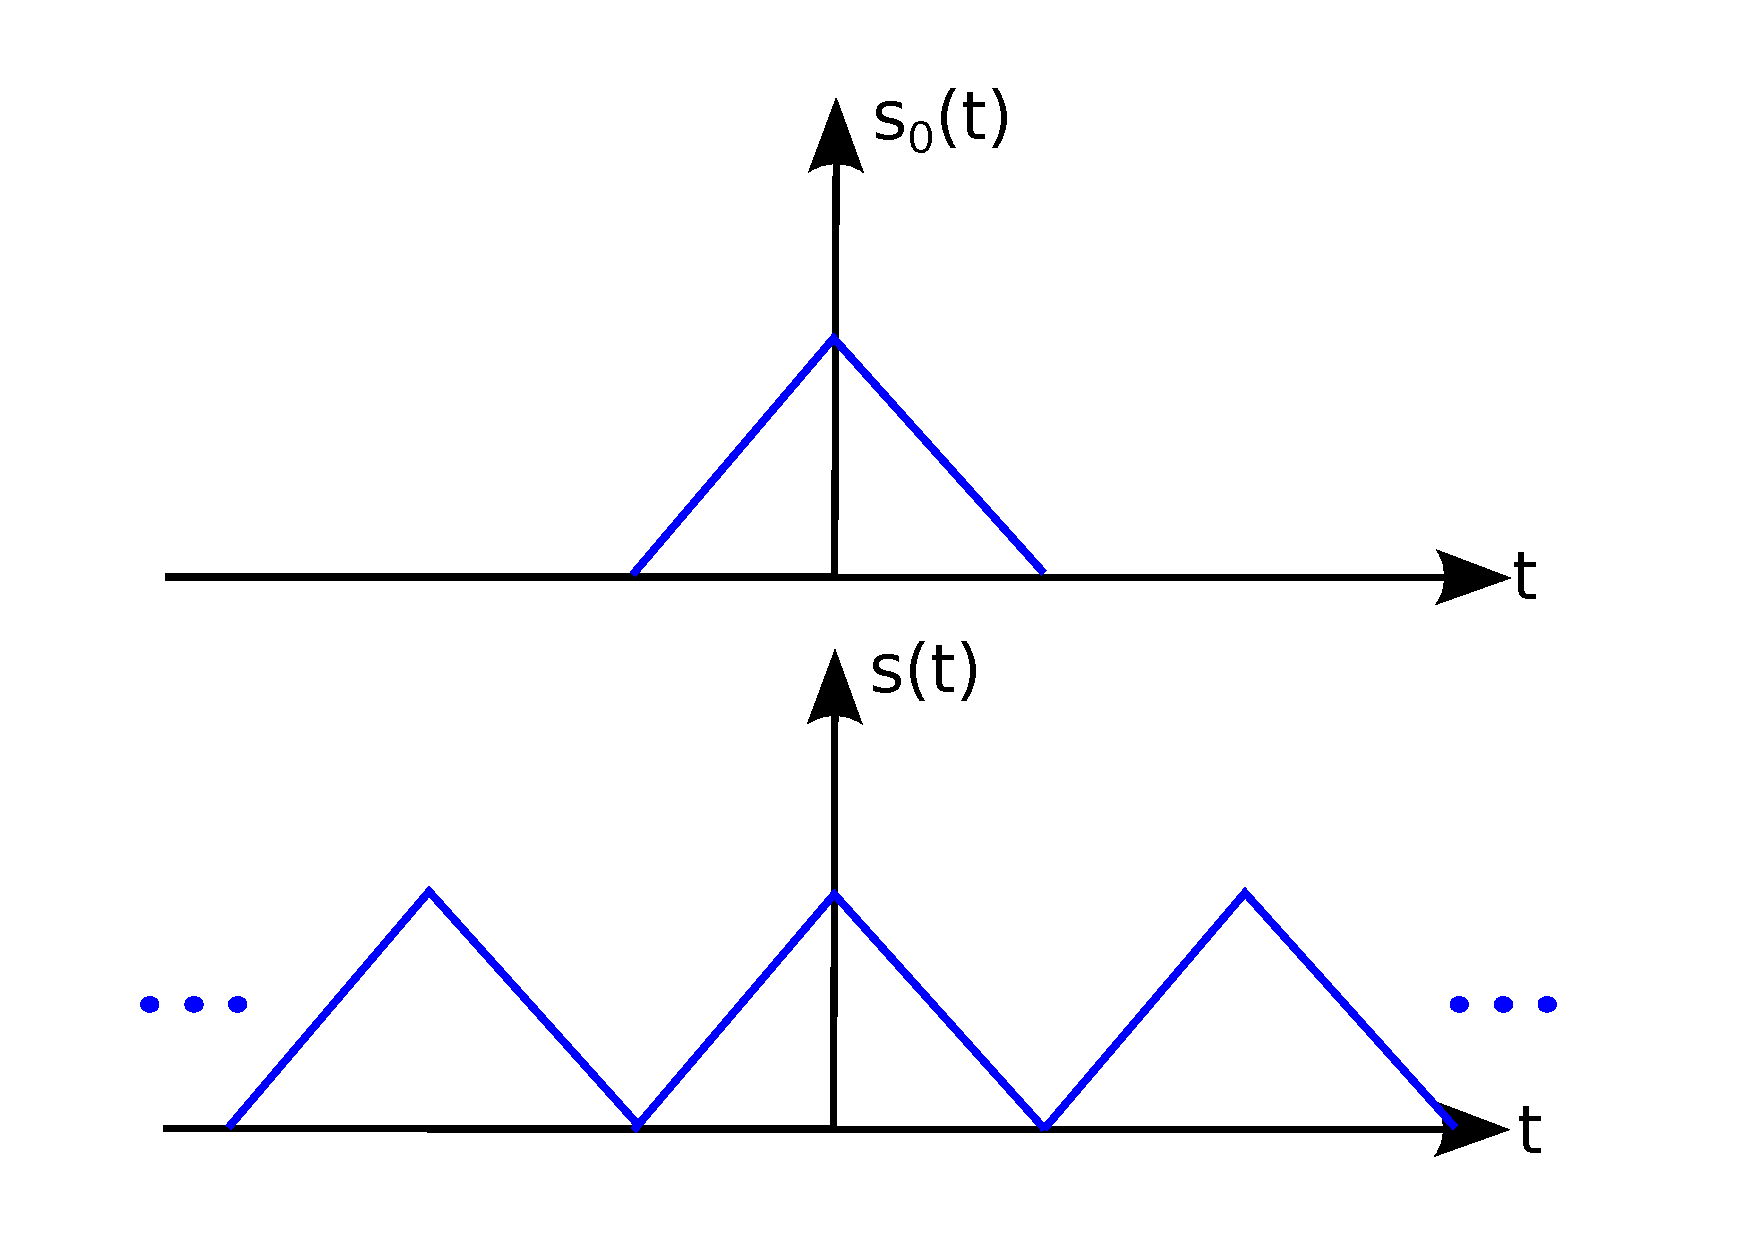
\includegraphics[width=0.25\textwidth]{content/appendix/FTperiodisch.pdf}} \\
$s(t) = \sum c_n \e^{jn\omega_0}$ dar. & \\
\end{tabular}	
